\documentclass{article}
\usepackage[utf8]{inputenc}
\usepackage{graphicx}
\usepackage{hyperref}

\title{Final Assignment: Integration of Tools and Practices}
\author{Amin Eslamian}
\date{\today}

\begin{document}

\maketitle
\newpage
\tableofcontents
\newpage


\section{Git and GitHub}
\subsection{Repository Initialization and Commits}
At the  beginning i created the repository using Github, making sure to create a Readme file to edit it later.


Then i added a file with LaTex format called main.tex.
right now i am completing the LaTex document and I submit the changes to the main.tex file in my Git repository since i am using overleaf website as an editor for writing my LaTex document, in order to work easier!

After that i make a directory using Github user interface, the directory is .github/workflows, i add the Latex.yml file to the directory.


Then through the Github, in the main page of the repository, in the Release section under About i click on it and realease a new tag and set tag version to v1.0 and target to main.


then i check if the compile process is done correctely by going to Actions section.


and then i write the README file.


At the end i update the LaTeX source(e.g., main.tex)

\subsection{GitHub Actions for LaTeX Compilation}
About this i described in the last part. but in additon i will refer to a challenge i personally had. at first i copied the suggested writings that i got from an AI in the .yml file, but then it seemed to cause an issue, so i edited the .yml file to the one that Mr.Zarei had uploded and the issue was fixed!

\section{Exploration Tasks}
\subsection{Vim Advanced Features}
\begin{enumerate}
    \item Text Objects with Custom Patterns

Define custom text objects using regex to manipulate specific patterns (e.g., Markdown links or XML tags).

Example: Create a mapping to select text inside Markdown links.

Why: Saves time when working with structured or repetitive text.

\item Expression Registers

Use the = register to evaluate Vimscript or shell commands and insert the result.

Example: Ctrl-R =2+2 inserts 4, or Ctrl-R =system('date') inserts the current date.

Why: Dynamically generate and insert content like calculations or timestamps.

\item Abbreviations with Execution

Use :abbreviate with :expr to execute Vimscript when an abbreviation is triggered.

Example: iabbrev <expr> dts strftime("%Y-%m-%d") inserts the current date when typing dts.

Why: Automate repetitive tasks like inserting boilerplate or dynamic content.
\end{enumerate}

\subsection{Memory Profiling}
\subsubsection{Memory Leak}

A memory leak happens when a program allocates memory but fails to release it after it’s no longer needed, causing unused memory to pile up and potentially slow down or crash the program.

\textbf{How Memory Leaks Happen}
\begin{enumerate}
    \item Forgotten Deallocation:

In languages like C, you allocate memory (e.g., malloc) but forget to free it (e.g., free).

\item Unreachable Objects:

In garbage-collected languages (e.g., Java, Python), objects are no longer needed but still referenced, so the garbage collector can’t reclaim them.

\item Circular References:

Objects reference each other, making them unreachable even when unused.

\item Unclosed Resources:

Failing to close files, databases, or network connections.
\end{enumerate}

\subsubsection{Memory Profilers}
A memory leak happens when a program allocates memory but fails to release it after it’s no longer needed, causing unused memory to pile up and potentially slow down or crash the program.


\textbf{How Memory Leaks Happen}
\begin{enumerate}
    \item Forgotten Deallocation:

In languages like C/C++, you allocate memory (e.g., malloc) but forget to free it (e.g., free).

\item Unreachable Objects:

In garbage-collected languages (e.g., Java, Python), objects are no longer needed but still referenced, so the garbage collector can’t reclaim them.

\item Circular References:

Objects reference each other, making them unreachable even when unused.

\item Unclosed Resources:

Failing to close files, databases, or network connections.
\end{enumerate}

\subsection{GNU/Linux Bash Scripting}
\subsubsection{fzf}
Read about a handy CLI tool called fzf and answer the following questions:
\begin{itemize}
    \item What is fuzzy searching? 

    Fuzzy searching is a technique that finds matches for a query even if the characters are not in exact order or are incomplete. It’s flexible and helps quickly narrow down results.
    
    \item A description of what the following command does: \texttt{ls | fzf}

    ls lists files/directories in the current directory.

fzf takes this list and lets you interactively fuzzy-search through it.

It’s a fast way to find and select files!
\end{itemize}

\subsubsection{Using fzf to find your favorite PDF}
\begin{enumerate}
    \item fd -e pdf

    \item fd -e pdf | fzf
\end{enumerate}

\subsubsection{Opening the file using Zathura}
zathura  \$(fd -e pdf  |  fzf)
\section{Git and FOSS}
\subsection{README.md}
Check out the README file in my repository!

\subsection{Issues}
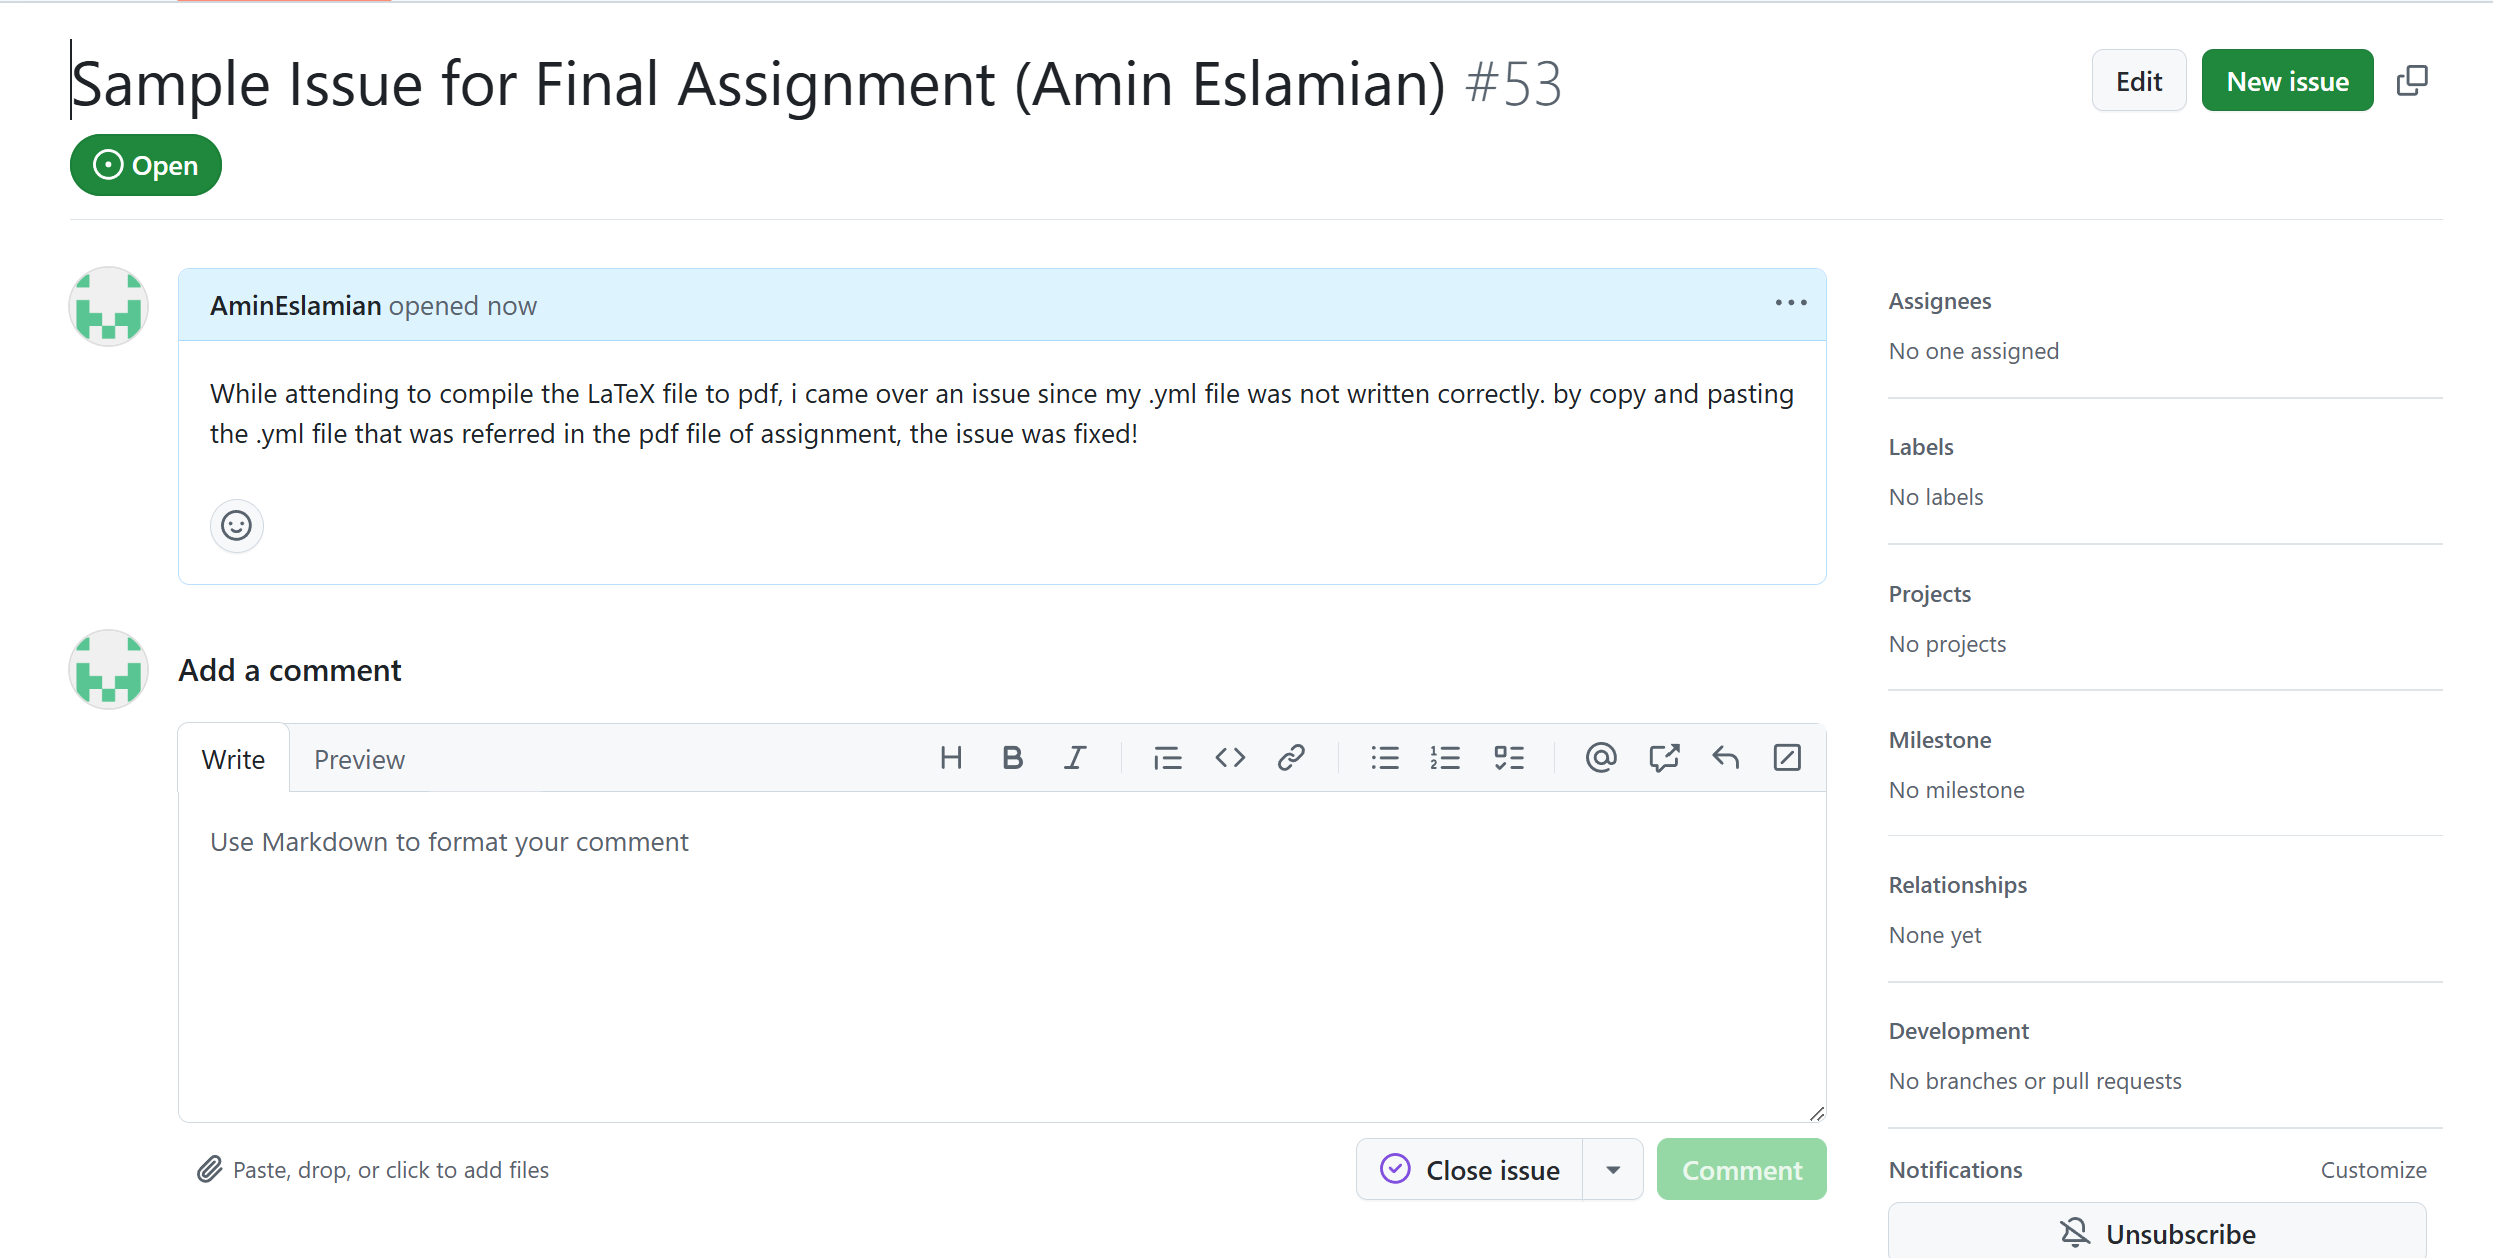
\includegraphics[width=1\textwidth]{issue_screen.png}

\subsection{FOSS contribution}
Yes because it's cool and it helps me do whatever i want, despite it's hard, it's worth it!

\end{document}
